%%%%%%%%%%%%%%%%%%%%%%%%%%%%%%%%%%%%%%%%%%%%%%%%%%%%%%%%%%%%%%%%%%%%%%%%%%%%%%%%%%
\begin{frame}[fragile]\frametitle{}
\begin{center}
{\Large Introduction}
\end{center}
\end{frame}

%%%%%%%%%%%%%%%%%%%%%%%%%%%%%%%%%%%%%%%%%%%%%%%%%%%%%%%%%%%%%%%%%%%%%%%%%%%%%%%%%%
\begin{frame}[fragile]\frametitle{What is Reinforcement Learning?}
Reinforcement Learning(RL) is a type of machine learning technique that enables an agent to learn in an interactive environment by trial and error using feedback from its own actions and experiences, to maximize cumulative rewards.


\end{frame}

%%%%%%%%%%%%%%%%%%%%%%%%%%%%%%%%%%%%%%%%%%%%%%%%%%%%%%%%%%%%%%%%%%%%%%%%%%%%%%%%%%
\begin{frame}[fragile]\frametitle{Real World Example}

\begin{columns}
\begin{column}{0.5\textwidth}

\begin{itemize}
\item A shop sells ice cream
\item Customers coming to shop can be random (stochastic), so shop owner finds it difficult to know how much stock to keep.
\item If stock is kept less, then all customers can not be served, so loss of business/income.
\item If stock is kept more, then wastage, so loss of business/income.
\item What's the optimum stock to maximize profit? Say, in a quarter.
\end{itemize}

\end{column}
\begin{column}{0.5\textwidth}  %%<--- here


\begin{center}
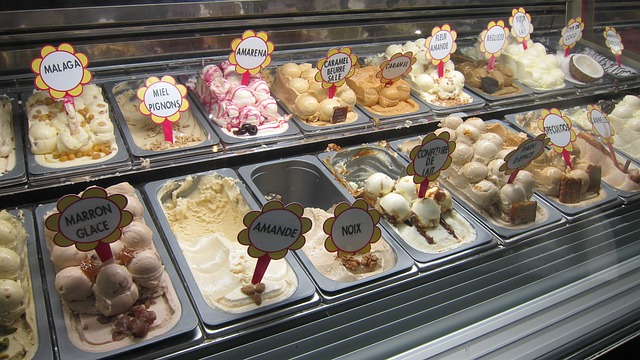
\includegraphics[width=0.8\linewidth,keepaspectratio]{rl56}
\end{center}
\end{column}
\end{columns}

\end{frame}


%%%%%%%%%%%%%%%%%%%%%%%%%%%%%%%%%%%%%%%%%%%%%%%%%%%%%%%%%%%%%%%%%%%%%%%%%%%%%%%%%%
\begin{frame}[fragile]\frametitle{Reinforcement Learning way}

\begin{itemize}
\item Agent: Shop owner, as he Acts
\item Environment: shop, shopkeeper, customers, stock, etc. even things like, 'demand'.
\item Action: how much to order from supplier to keep as stock for that day?
\item Reward: cumulative profits over the quarter. Its 'expected' as customer demand is stochastic.
\end{itemize}
Goal: how much to stock daily so as to maximize expected quarterly profits
\end{frame}

%%%%%%%%%%%%%%%%%%%%%%%%%%%%%%%%%%%%%%%%%%%%%%%%%%%%%%%%%%%%%%%%%%%%%%%%%%%%%%%%%%
\begin{frame}[fragile]\frametitle{Reinforcement Learning Visual way}

\begin{columns}
\begin{column}{0.5\textwidth}

\begin{itemize}
\item Circle is State of the Environment, has attributes like stock, weather, etc
\item Action emanates from it become next State. Action can be of ordering 2/5/10 crates of ice creams. The next state has that attribute updated.
\item Reward is shown on arrow line.
\item Out of two specific paths shown, best (blue) is the winner path of maximizing the profits.
\item $---$ means similar Actions.
\end{itemize}

\end{column}
\begin{column}{0.5\textwidth}  %%<--- here


\begin{center}
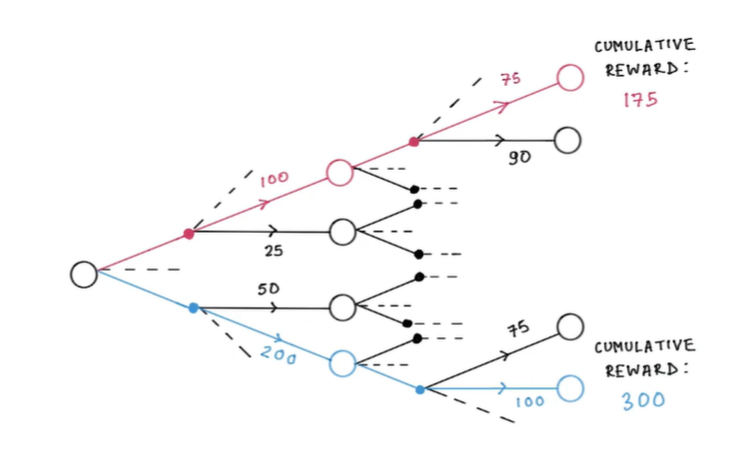
\includegraphics[width=0.8\linewidth,keepaspectratio]{rl57}

{\tiny (Ref: Fast RL course - Dibya Chakraborty)}

\end{center}
\end{column}
\end{columns}



\end{frame}

%%%%%%%%%%%%%%%%%%%%%%%%%%%%%%%%%%%%%%%%%%%%%%%%%%%%%%%%%%%%%%%%%%%%%%%%%%%%%%%%%%
\begin{frame}[fragile]\frametitle{RL Applications}
 Not just for forecasting demand for ice cream but:
\begin{itemize}
\item Energy usage reduction in data centers.
\item Managing feet of vehicles
\item Stock trading
\item Games
\item Robotics
\item Autonomous cars
\end{itemize}

Typically, Control-Feedback based Sequential Decision making tasks.

\end{frame}


%%%%%%%%%%%%%%%%%%%%%%%%%%%%%%%%%%%%%%%%%%%%%%%%%%%%%%%%%%%%%%%%%%%%%%%%%%%%%%%%%%
\begin{frame}[fragile]\frametitle{ML vs RL}

\begin{itemize}
\item In supervised ML: labels ie correct answers are known upfront, eg. for prediction if image is cat or a dog, hundreds of cats and dogs images have to be provided for training.
\item In Reinforcement Learning,  nothing is known upfront. Need to act first, then you get some reward. The training is to decide such actions that gives probability of more rewards. Trial and Error. Being stochastic, same action may not result in same reward.
\end{itemize}
\end{frame}

%%%%%%%%%%%%%%%%%%%%%%%%%%%%%%%%%%%%%%%%%%%%%%%%%%%%%%%%%%%%%%%%%%%%%%%%%%%%%%%%%%
\begin{frame}[fragile]\frametitle{ML vs RL}

\begin{columns}
\begin{column}{0.5\textwidth}

\begin{itemize}
\item In supervised ML data is i.i.d (identical and independently distributed data), means, each data (row) is independent of any part/previous data. 
\item In Reinforcement Learning, State may depend on previous State. Even if some actions may result in lesser immediate rewards, in the long run they may turn out to be the best. Because, some intermediate states can be better or worse. Long Term Thinking, Strategy with harmonized/coordinated Actions.
\end{itemize}

\end{column}
\begin{column}{0.5\textwidth}  %%<--- here


\begin{center}
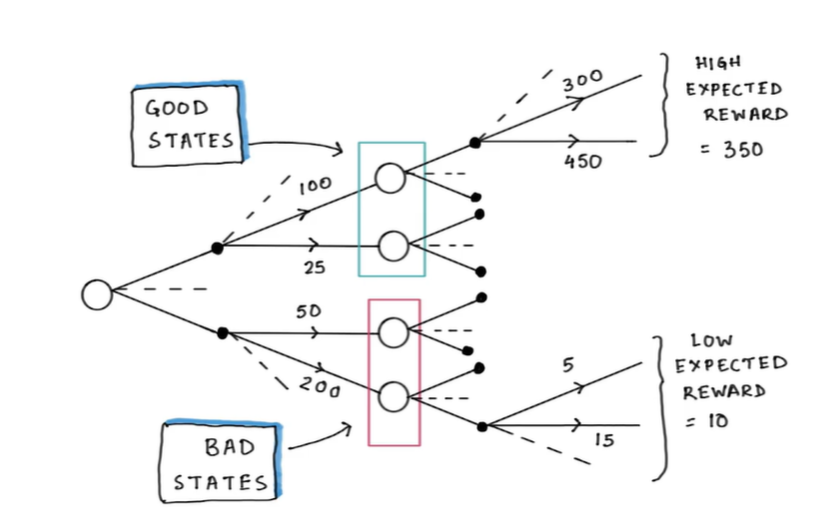
\includegraphics[width=0.8\linewidth,keepaspectratio]{rl58}

{\tiny (Ref: Fast RL course - Dibya Chakraborty)}

\end{center}
\end{column}
\end{columns}

\end{frame}


%%%%%%%%%%%%%%%%%%%%%%%%%%%%%%%%%%%%%%%%%%%%%%%%%%%%%%%%%%%%%%%%%%%%%%%%%%%%%%%%%%
\begin{frame}[fragile]\frametitle{ML vs RL}

No labeled data needed but just nudging whether model is in right direction or not. Outcome is a policy (recipe) for success.

\begin{center}
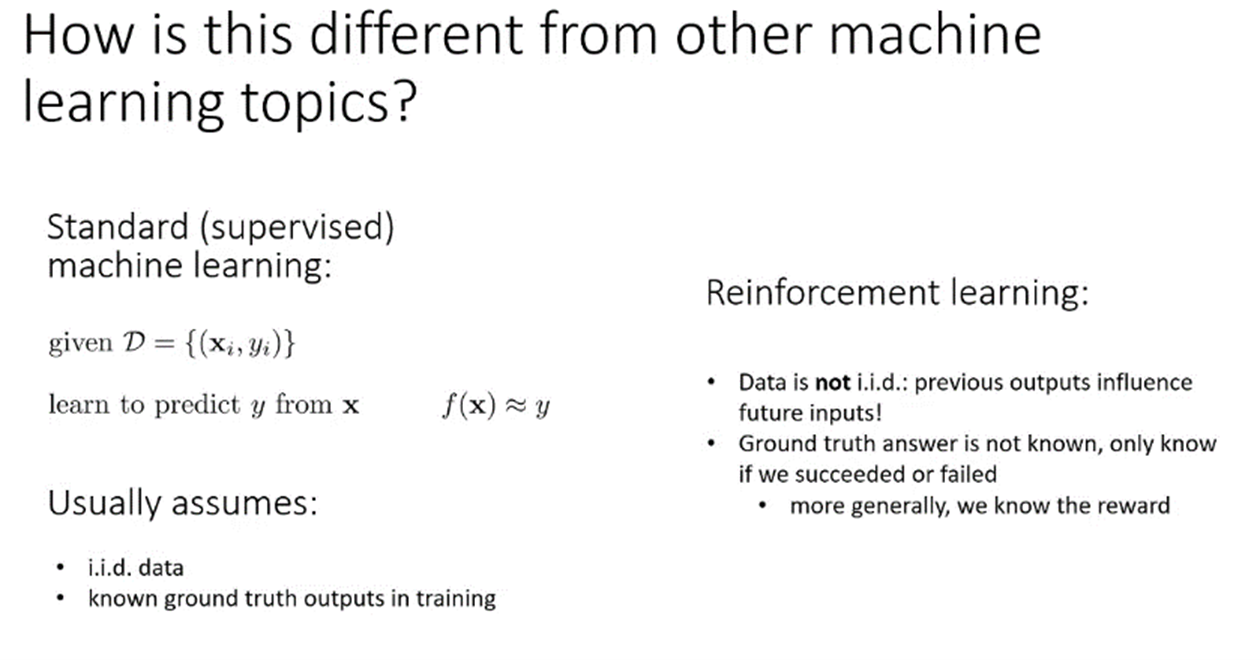
\includegraphics[width=0.8\linewidth,keepaspectratio]{rl45}
\end{center}

{\tiny (Ref: CS 285 Fall 2020 Deep Reinforcement Learning)}

\end{frame}

%%%%%%%%%%%%%%%%%%%%%%%%%%%%%%%%%%%%%%%%%%%%%%%%%%%%%%%%%%%%%%%%%%%%%%%%%%%%%%%%%%
\begin{frame}[fragile]\frametitle{Deep Learning}

Deep Learning replaced Machine Learning by automatically discovering features. Similarity, a classical RL would need to device features, policies or value table etc to come up with next action. Deep RL automates this all.

\begin{center}
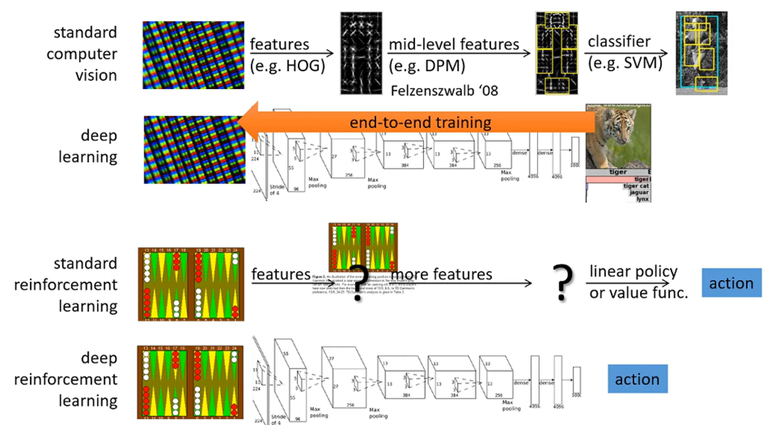
\includegraphics[width=0.8\linewidth,keepaspectratio]{rl46}
\end{center}


{\tiny (Ref: CS 285 Fall 2020 Deep Reinforcement Learning)}

\end{frame}


%%%%%%%%%%%%%%%%%%%%%%%%%%%%%%%%%%%%%%%%%%%%%%%%%%%%%%%%%%%%%%%%%%%%%%%%%%%%%%%%%%
\begin{frame}[fragile]\frametitle{Deep Learning}

End-to-End system does not do stage wise recognition, meaning, image recognition first then action prediction, but does everything in a single go.

\begin{center}
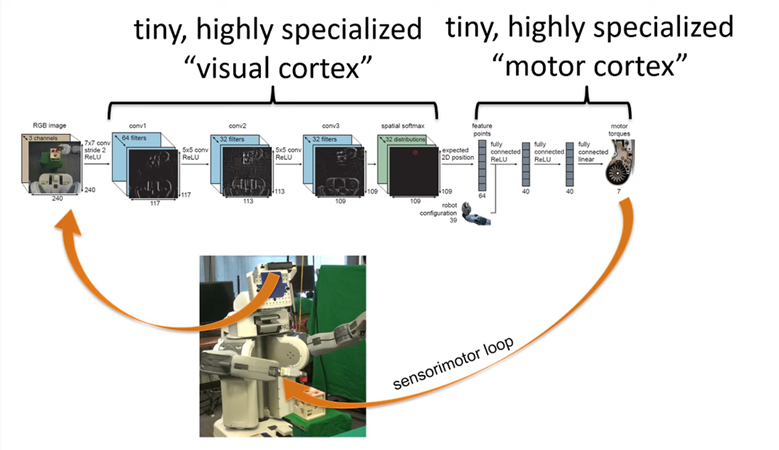
\includegraphics[width=0.8\linewidth,keepaspectratio]{rl47}
\end{center}


{\tiny (Ref: CS 285 Fall 2020 Deep Reinforcement Learning)}

\end{frame}

%%%%%%%%%%%%%%%%%%%%%%%%%%%%%%%%%%%%%%%%%%%%%%%%%%%%%%%%%%%%%%%%%%%%%%%%%%%%%%%%%%
\begin{frame}[fragile]\frametitle{Deep Learning a step towards Artificial General Intelligence?}

\begin{itemize}
\item Deep Learning perceives and represents environment/data well but can bot deal with long term planning, strategy, etc.
\item Reinforcement Learning is good at long term planning, strategy, etc.
\item Combining both can be close to better intelligence. 
\end{itemize}

\end{frame}

%%%%%%%%%%%%%%%%%%%%%%%%%%%%%%%%%%%%%%%%%%%%%%%%%%%%%%%%%%%%%%%%%%%%%%%%%%%%%%%%%%
\begin{frame}[fragile]\frametitle{To RL or not to RL?}

\begin{itemize}
\item Difficult to tell the correct action before actually executing it (and getting reward) but easy to score once taken.
\item Is current data/state dependent on previous data/state?
\item Cumulative Reward more important than the immediate ones.
\end{itemize}
\end{frame}

%%%%%%%%%%%%%%%%%%%%%%%%%%%%%%%%%%%%%%%%%%%%%%%%%%%%%%%%%%%%%%%%%%%%%%%%%%%%%%%%%%
\begin{frame}[fragile]\frametitle{How to RL?}

\begin{itemize}
\item As we are doing trial and errors, you can not try them in real life (autonomous car?), so a simulation is used to try and train RL, virtual shop, virtual car, etc.
\item Approximately model, key interactions, states, rewards, stochastic inputs, actions, etc.
\item Once proven ok, can be deployed in the real world.
\item So, there are two things in any RL problem
\item Simulation $==$ Environment
\item RL algorithm/Library $==$ Agent.
\end{itemize}
\end{frame}

%%%%%%%%%%%%%%%%%%%%%%%%%%%%%%%%%%%%%%%%%%%%%%%%%%%%%%%%%%%%%%%%%%%%%%%%%%%%%%%%%%
\begin{frame}[fragile]\frametitle{How RL Algorithms work?}

Famous RL Algorithms:
\begin{itemize}
\item Deep Q Network (DQN): Atari video games
\item Proximal Policy Optimization (PPO): DOTA 2
\item Although used in games, RL algorithms are generic and more or less similar.
\end{itemize}

At High level:
\begin{itemize}
\item At start Agent (RL Algorithm) starts with random actions (exploration) to find out their consequent immediate reward and next state. So, Policy here is $\pi(a|s) = random()$ So paths are random. So, low cumulative awards.
\item During exploration, the Agent gathers Experiences, ie $(S,a,S',r_{SS'}^a)$ tuples.
\item Once enough experiences are gathered, they start getting used to decide the next action, with an updated policy $\pi_1$. This is Exploitation and has better Expected cumulative rewards.
\item This goes on, ie more experience, updated policy $\pi_2$ and so on, till the policy does not improve anymore.
\end{itemize}
\end{frame}

%%%%%%%%%%%%%%%%%%%%%%%%%%%%%%%%%%%%%%%%%%%%%%%%%%%%%%%%%%%%%%%%%%%%%%%%%%%%%%%%%%
\begin{frame}[fragile]\frametitle{How RL Algorithms work?}

\begin{center}
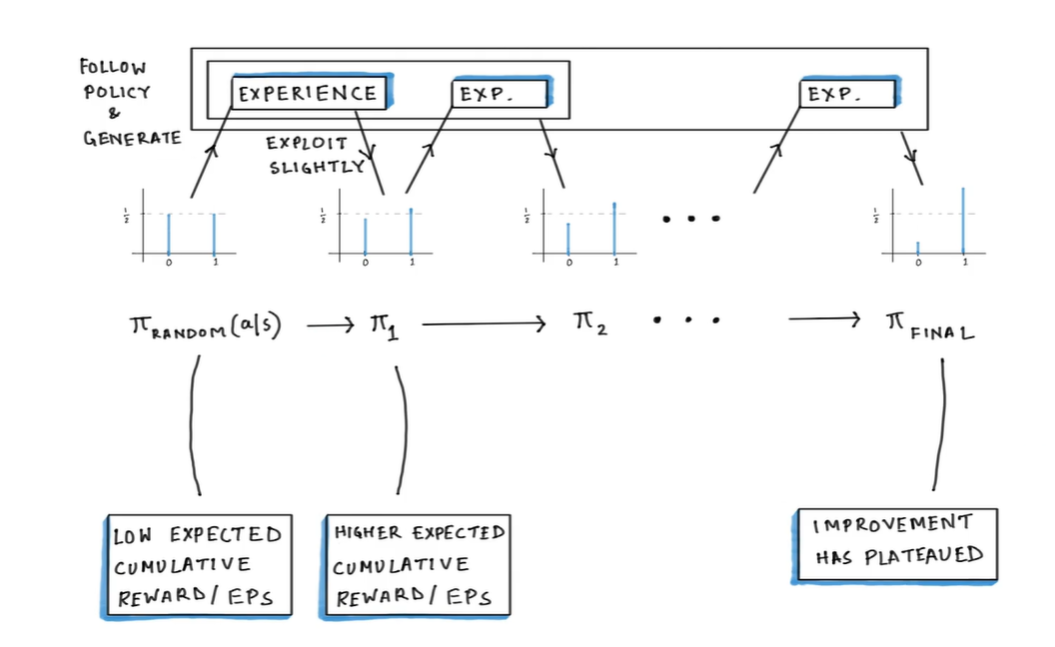
\includegraphics[width=0.8\linewidth,keepaspectratio]{rl62}

{\tiny (Ref: Fast RL course - Dibya Chakraborty)}
\end{center}

\end{frame}


%%%%%%%%%%%%%%%%%%%%%%%%%%%%%%%%%%%%%%%%%%%%%%%%%%%%%%%%%%%%%%%%%%%%%%%%%%%%%%%%%%
\begin{frame}[fragile]\frametitle{How RL Algorithms work?}

\begin{center}
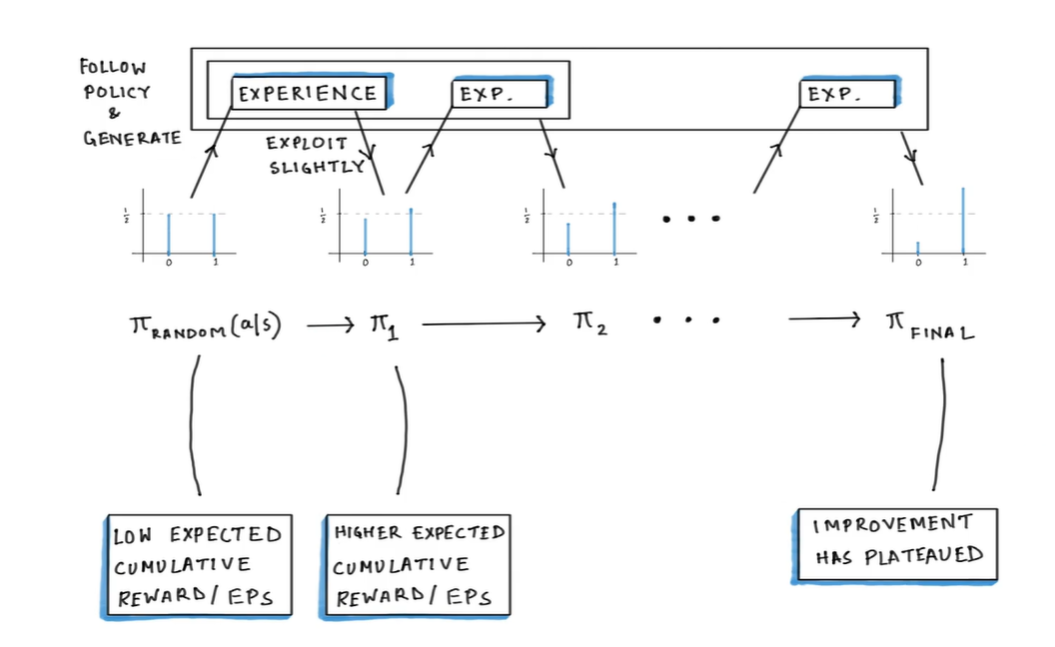
\includegraphics[width=0.4\linewidth,keepaspectratio]{rl62}

{\tiny (Ref: Fast RL course - Dibya Chakraborty)}
\end{center}

\begin{itemize}
\item Note how the final policy is very different from the initial ones, but deltas among neighbors is small.
\item For continuous rewards, there is probability distribution, instead of discrete values.
\item This process is ok for small state spaces, but not for millions, like in Atari game, it goes in millions. 
\item Solution: Deep RL: Neural Network takes state as input and outputs some quantity useful for exploitation.
\item RL Algorithms structure is same but how they update the policy based on experiences, differ.
\end{itemize}
\end{frame}

%%%%%%%%%%%%%%%%%%%%%%%%%%%%%%%%%%%%%%%%%%%%%%%%%%%%%%%%%%%%%%%%%%%%%%%%%%%%%%%%%%
\begin{frame}[fragile]\frametitle{RL Libs}

\begin{itemize}
\item Libraries like `rllib` have production have implementations of Deep RL algorithms.
\item High level APIs abstract the details
\item E.g. often the solution is stated as : `` Use DQN on Cart Pole' where CartPole is Environment and DQN is the algorithm.
\end{itemize}

Comparison of RL frameworks:

\begin{center}
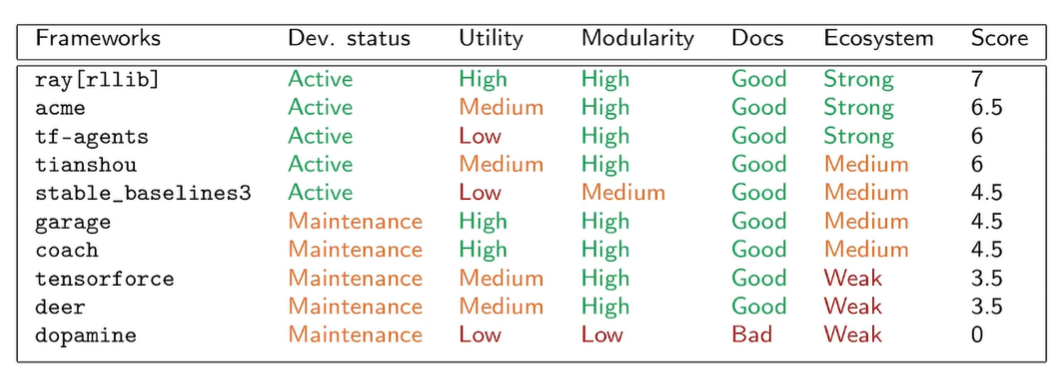
\includegraphics[width=0.8\linewidth,keepaspectratio]{rl63}

{\tiny (Ref: Fast RL course - Dibya Chakraborty)}
\end{center}

\end{frame}